\documentclass[twoside]{book}

% Packages required by doxygen
\usepackage{fixltx2e}
\usepackage{calc}
\usepackage{doxygen}
\usepackage[export]{adjustbox} % also loads graphicx
\usepackage{graphicx}
\usepackage[utf8]{inputenc}
\usepackage{makeidx}
\usepackage{multicol}
\usepackage{multirow}
\PassOptionsToPackage{warn}{textcomp}
\usepackage{textcomp}
\usepackage[nointegrals]{wasysym}
\usepackage[table]{xcolor}

% Font selection
\usepackage[T1]{fontenc}
\usepackage[scaled=.90]{helvet}
\usepackage{courier}
\usepackage{amssymb}
\usepackage{sectsty}
\renewcommand{\familydefault}{\sfdefault}
\allsectionsfont{%
  \fontseries{bc}\selectfont%
  \color{darkgray}%
}
\renewcommand{\DoxyLabelFont}{%
  \fontseries{bc}\selectfont%
  \color{darkgray}%
}
\newcommand{\+}{\discretionary{\mbox{\scriptsize$\hookleftarrow$}}{}{}}

% Page & text layout
\usepackage{geometry}
\geometry{%
  a4paper,%
  top=2.5cm,%
  bottom=2.5cm,%
  left=2.5cm,%
  right=2.5cm%
}
\tolerance=750
\hfuzz=15pt
\hbadness=750
\setlength{\emergencystretch}{15pt}
\setlength{\parindent}{0cm}
\setlength{\parskip}{3ex plus 2ex minus 2ex}
\makeatletter
\renewcommand{\paragraph}{%
  \@startsection{paragraph}{4}{0ex}{-1.0ex}{1.0ex}{%
    \normalfont\normalsize\bfseries\SS@parafont%
  }%
}
\renewcommand{\subparagraph}{%
  \@startsection{subparagraph}{5}{0ex}{-1.0ex}{1.0ex}{%
    \normalfont\normalsize\bfseries\SS@subparafont%
  }%
}
\makeatother

% Headers & footers
\usepackage{fancyhdr}
\pagestyle{fancyplain}
\fancyhead[LE]{\fancyplain{}{\bfseries\thepage}}
\fancyhead[CE]{\fancyplain{}{}}
\fancyhead[RE]{\fancyplain{}{\bfseries\leftmark}}
\fancyhead[LO]{\fancyplain{}{\bfseries\rightmark}}
\fancyhead[CO]{\fancyplain{}{}}
\fancyhead[RO]{\fancyplain{}{\bfseries\thepage}}
\fancyfoot[LE]{\fancyplain{}{}}
\fancyfoot[CE]{\fancyplain{}{}}
\fancyfoot[RE]{\fancyplain{}{\bfseries\scriptsize Generated by Doxygen }}
\fancyfoot[LO]{\fancyplain{}{\bfseries\scriptsize Generated by Doxygen }}
\fancyfoot[CO]{\fancyplain{}{}}
\fancyfoot[RO]{\fancyplain{}{}}
\renewcommand{\footrulewidth}{0.4pt}
\renewcommand{\chaptermark}[1]{%
  \markboth{#1}{}%
}
\renewcommand{\sectionmark}[1]{%
  \markright{\thesection\ #1}%
}

% Indices & bibliography
\usepackage{natbib}
\usepackage[titles]{tocloft}
\setcounter{tocdepth}{3}
\setcounter{secnumdepth}{5}
\makeindex

% Hyperlinks (required, but should be loaded last)
\usepackage{ifpdf}
\ifpdf
  \usepackage[pdftex,pagebackref=true]{hyperref}
\else
  \usepackage[ps2pdf,pagebackref=true]{hyperref}
\fi
\hypersetup{%
  colorlinks=true,%
  linkcolor=blue,%
  citecolor=blue,%
  unicode%
}

% Custom commands
\newcommand{\clearemptydoublepage}{%
  \newpage{\pagestyle{empty}\cleardoublepage}%
}

\usepackage{caption}
\captionsetup{labelsep=space,justification=centering,font={bf},singlelinecheck=off,skip=4pt,position=top}

%===== C O N T E N T S =====

\begin{document}

% Titlepage & ToC
\hypersetup{pageanchor=false,
             bookmarksnumbered=true,
             pdfencoding=unicode
            }
\pagenumbering{alph}
\begin{titlepage}
\vspace*{7cm}
\begin{center}%
{\Large Lab1 }\\
\vspace*{1cm}
{\large Generated by Doxygen 1.8.13}\\
\end{center}
\end{titlepage}
\clearemptydoublepage
\pagenumbering{roman}
\tableofcontents
\clearemptydoublepage
\pagenumbering{arabic}
\hypersetup{pageanchor=true}

%--- Begin generated contents ---
\chapter{Hierarchical Index}
\section{Class Hierarchy}
This inheritance list is sorted roughly, but not completely, alphabetically\+:\begin{DoxyCompactList}
\item \contentsline{section}{lab\+:\+:impl\+:\+:I\+Queue$<$ T $>$}{\pageref{classlab_1_1impl_1_1IQueue}}{}
\begin{DoxyCompactList}
\item \contentsline{section}{lab\+:\+:impl\+:\+:Dynamic\+Array\+Queue$<$ T $>$}{\pageref{classlab_1_1impl_1_1DynamicArrayQueue}}{}
\item \contentsline{section}{lab\+:\+:impl\+:\+:Linked\+List\+Queue$<$ T $>$}{\pageref{classlab_1_1impl_1_1LinkedListQueue}}{}
\item \contentsline{section}{lab\+:\+:impl\+:\+:Static\+Array\+Queue$<$ T, Size $>$}{\pageref{classlab_1_1impl_1_1StaticArrayQueue}}{}
\end{DoxyCompactList}
\item \contentsline{section}{lab\+:\+:impl\+:\+:Storage\+Selector$<$ storage $>$}{\pageref{structlab_1_1impl_1_1StorageSelector}}{}
\item \contentsline{section}{lab\+:\+:impl\+:\+:Storage\+Selector$<$ Storage\+:\+:Dynamic $>$}{\pageref{structlab_1_1impl_1_1StorageSelector_3_01Storage_1_1Dynamic_01_4}}{}
\item \contentsline{section}{lab\+:\+:impl\+:\+:Storage\+Selector$<$ Storage\+:\+:Linked\+List $>$}{\pageref{structlab_1_1impl_1_1StorageSelector_3_01Storage_1_1LinkedList_01_4}}{}
\item \contentsline{section}{lab\+:\+:impl\+:\+:Storage\+Selector$<$ Storage\+:\+:Static $>$}{\pageref{structlab_1_1impl_1_1StorageSelector_3_01Storage_1_1Static_01_4}}{}
\item template storage\+\_\+type$<$ T, Size\+For\+Static\+Storage... $>$\begin{DoxyCompactList}
\item \contentsline{section}{lab\+:\+:Queue$<$ T, Storage\+Type, Size\+For\+Static\+Storage $>$}{\pageref{classlab_1_1Queue}}{}
\end{DoxyCompactList}
\item \contentsline{section}{lab\+:\+:impl\+:\+:Undefined\+Storage}{\pageref{classlab_1_1impl_1_1UndefinedStorage}}{}
\end{DoxyCompactList}

\chapter{Class Index}
\section{Class List}
Here are the classes, structs, unions and interfaces with brief descriptions\+:\begin{DoxyCompactList}
\item\contentsline{section}{\hyperlink{classlab_1_1impl_1_1DynamicArrayQueue}{lab\+::impl\+::\+Dynamic\+Array\+Queue$<$ T $>$} \\*Class that holds queue implementation based on std\+::vector {\bfseries Operations} complexity\+: }{\pageref{classlab_1_1impl_1_1DynamicArrayQueue}}{}
\item\contentsline{section}{\hyperlink{classlab_1_1impl_1_1IQueue}{lab\+::impl\+::\+I\+Queue$<$ T $>$} \\*Interface for queue implementations }{\pageref{classlab_1_1impl_1_1IQueue}}{}
\item\contentsline{section}{\hyperlink{classlab_1_1impl_1_1LinkedListQueue}{lab\+::impl\+::\+Linked\+List\+Queue$<$ T $>$} \\*Class that holds queue implementation based on std\+::list {\bfseries Operations} complexity\+: }{\pageref{classlab_1_1impl_1_1LinkedListQueue}}{}
\item\contentsline{section}{\hyperlink{classlab_1_1Queue}{lab\+::\+Queue$<$ T, Storage\+Type, Size\+For\+Static\+Storage $>$} \\*Class with queue implementation based on {\ttfamily Storage\+Type} }{\pageref{classlab_1_1Queue}}{}
\item\contentsline{section}{\hyperlink{classlab_1_1impl_1_1StaticArrayQueue}{lab\+::impl\+::\+Static\+Array\+Queue$<$ T, Size $>$} \\*Class that holds queue implementation based on std\+::array {\bfseries Operations} complexity\+: }{\pageref{classlab_1_1impl_1_1StaticArrayQueue}}{}
\item\contentsline{section}{\hyperlink{structlab_1_1impl_1_1StorageSelector}{lab\+::impl\+::\+Storage\+Selector$<$ storage $>$} }{\pageref{structlab_1_1impl_1_1StorageSelector}}{}
\item\contentsline{section}{\hyperlink{structlab_1_1impl_1_1StorageSelector_3_01Storage_1_1Dynamic_01_4}{lab\+::impl\+::\+Storage\+Selector$<$ Storage\+::\+Dynamic $>$} }{\pageref{structlab_1_1impl_1_1StorageSelector_3_01Storage_1_1Dynamic_01_4}}{}
\item\contentsline{section}{\hyperlink{structlab_1_1impl_1_1StorageSelector_3_01Storage_1_1LinkedList_01_4}{lab\+::impl\+::\+Storage\+Selector$<$ Storage\+::\+Linked\+List $>$} }{\pageref{structlab_1_1impl_1_1StorageSelector_3_01Storage_1_1LinkedList_01_4}}{}
\item\contentsline{section}{\hyperlink{structlab_1_1impl_1_1StorageSelector_3_01Storage_1_1Static_01_4}{lab\+::impl\+::\+Storage\+Selector$<$ Storage\+::\+Static $>$} }{\pageref{structlab_1_1impl_1_1StorageSelector_3_01Storage_1_1Static_01_4}}{}
\item\contentsline{section}{\hyperlink{classlab_1_1impl_1_1UndefinedStorage}{lab\+::impl\+::\+Undefined\+Storage} }{\pageref{classlab_1_1impl_1_1UndefinedStorage}}{}
\end{DoxyCompactList}

\chapter{Class Documentation}
\hypertarget{classlab_1_1impl_1_1DynamicArrayQueue}{}\section{lab\+:\+:impl\+:\+:Dynamic\+Array\+Queue$<$ T $>$ Class Template Reference}
\label{classlab_1_1impl_1_1DynamicArrayQueue}\index{lab\+::impl\+::\+Dynamic\+Array\+Queue$<$ T $>$@{lab\+::impl\+::\+Dynamic\+Array\+Queue$<$ T $>$}}


Class that holds queue implementation based on std\+::vector {\bfseries Operations} complexity\+:  




{\ttfamily \#include $<$Dynamic\+Array.\+hpp$>$}



Inheritance diagram for lab\+:\+:impl\+:\+:Dynamic\+Array\+Queue$<$ T $>$\+:
\nopagebreak
\begin{figure}[H]
\begin{center}
\leavevmode
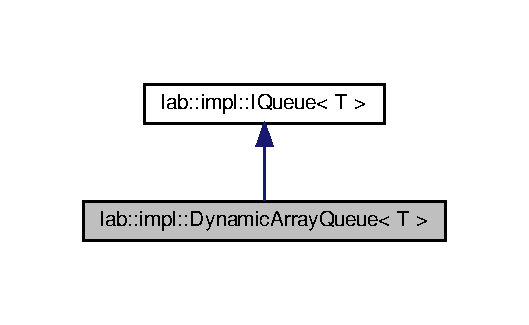
\includegraphics[width=254pt]{classlab_1_1impl_1_1DynamicArrayQueue__inherit__graph}
\end{center}
\end{figure}


Collaboration diagram for lab\+:\+:impl\+:\+:Dynamic\+Array\+Queue$<$ T $>$\+:
\nopagebreak
\begin{figure}[H]
\begin{center}
\leavevmode
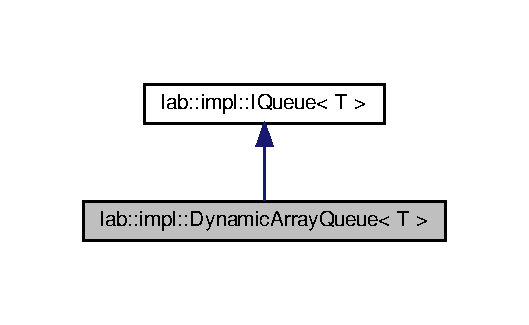
\includegraphics[width=254pt]{classlab_1_1impl_1_1DynamicArrayQueue__coll__graph}
\end{center}
\end{figure}
\subsection*{Public Member Functions}
\begin{DoxyCompactItemize}
\item 
{\footnotesize template$<$typename... Ts$>$ }\\\hyperlink{classlab_1_1impl_1_1DynamicArrayQueue_a1c39ec156dd583bb102839d7b4eec5d6}{Dynamic\+Array\+Queue} (Ts \&\&... args)
\begin{DoxyCompactList}\small\item\em Constructs queue from arbitary number of args. \end{DoxyCompactList}\item 
\mbox{\Hypertarget{classlab_1_1impl_1_1DynamicArrayQueue_ad9efa241a1b44bcab089614fecfbd27b}\label{classlab_1_1impl_1_1DynamicArrayQueue_ad9efa241a1b44bcab089614fecfbd27b}} 
void \hyperlink{classlab_1_1impl_1_1DynamicArrayQueue_ad9efa241a1b44bcab089614fecfbd27b}{push} (const T \&value) override
\begin{DoxyCompactList}\small\item\em Inserts value to end of the queue. \end{DoxyCompactList}\item 
\mbox{\Hypertarget{classlab_1_1impl_1_1DynamicArrayQueue_a1ce4ca0bca46d2228c063aa22e031bff}\label{classlab_1_1impl_1_1DynamicArrayQueue_a1ce4ca0bca46d2228c063aa22e031bff}} 
void \hyperlink{classlab_1_1impl_1_1DynamicArrayQueue_a1ce4ca0bca46d2228c063aa22e031bff}{push} (T \&\&value) override
\begin{DoxyCompactList}\small\item\em Inserts value to end of the queue. \end{DoxyCompactList}\item 
\mbox{\Hypertarget{classlab_1_1impl_1_1DynamicArrayQueue_a5263af315b723598977cbe48395e624c}\label{classlab_1_1impl_1_1DynamicArrayQueue_a5263af315b723598977cbe48395e624c}} 
T \hyperlink{classlab_1_1impl_1_1DynamicArrayQueue_a5263af315b723598977cbe48395e624c}{pop} () override
\begin{DoxyCompactList}\small\item\em Removes first element in queue. \end{DoxyCompactList}\item 
\mbox{\Hypertarget{classlab_1_1impl_1_1DynamicArrayQueue_a1b944916c9b3a1b2c96a21e76e3aa4f0}\label{classlab_1_1impl_1_1DynamicArrayQueue_a1b944916c9b3a1b2c96a21e76e3aa4f0}} 
const T \& \hyperlink{classlab_1_1impl_1_1DynamicArrayQueue_a1b944916c9b3a1b2c96a21e76e3aa4f0}{front} () const override
\begin{DoxyCompactList}\small\item\em Returns first element in queue. \end{DoxyCompactList}\item 
\mbox{\Hypertarget{classlab_1_1impl_1_1DynamicArrayQueue_ad882a135dfde4d64fc00cd44c9cd0e5a}\label{classlab_1_1impl_1_1DynamicArrayQueue_ad882a135dfde4d64fc00cd44c9cd0e5a}} 
bool \hyperlink{classlab_1_1impl_1_1DynamicArrayQueue_ad882a135dfde4d64fc00cd44c9cd0e5a}{empty} () const noexcept override
\begin{DoxyCompactList}\small\item\em Returns true if queue is empty. \end{DoxyCompactList}\end{DoxyCompactItemize}
\subsection*{Additional Inherited Members}


\subsection{Detailed Description}
\subsubsection*{template$<$typename T$>$\newline
class lab\+::impl\+::\+Dynamic\+Array\+Queue$<$ T $>$}

Class that holds queue implementation based on std\+::vector {\bfseries Operations} complexity\+: 

\begin{DoxyItemize}
\item Push -\/ O(1) \item Pop -\/ O(1) \end{DoxyItemize}


\subsection{Constructor \& Destructor Documentation}
\mbox{\Hypertarget{classlab_1_1impl_1_1DynamicArrayQueue_a1c39ec156dd583bb102839d7b4eec5d6}\label{classlab_1_1impl_1_1DynamicArrayQueue_a1c39ec156dd583bb102839d7b4eec5d6}} 
\index{lab\+::impl\+::\+Dynamic\+Array\+Queue@{lab\+::impl\+::\+Dynamic\+Array\+Queue}!Dynamic\+Array\+Queue@{Dynamic\+Array\+Queue}}
\index{Dynamic\+Array\+Queue@{Dynamic\+Array\+Queue}!lab\+::impl\+::\+Dynamic\+Array\+Queue@{lab\+::impl\+::\+Dynamic\+Array\+Queue}}
\subsubsection{\texorpdfstring{Dynamic\+Array\+Queue()}{DynamicArrayQueue()}}
{\footnotesize\ttfamily template$<$typename T $>$ \\
template$<$typename... Ts$>$ \\
\hyperlink{classlab_1_1impl_1_1DynamicArrayQueue}{lab\+::impl\+::\+Dynamic\+Array\+Queue}$<$ T $>$\+::\hyperlink{classlab_1_1impl_1_1DynamicArrayQueue}{Dynamic\+Array\+Queue} (\begin{DoxyParamCaption}\item[{Ts \&\&...}]{args }\end{DoxyParamCaption})}



Constructs queue from arbitary number of args. 


\begin{DoxyParams}{Parameters}
{\em Args} & must be same type \\
\hline
\end{DoxyParams}


The documentation for this class was generated from the following file\+:\begin{DoxyCompactItemize}
\item 
/home/starquell/\+C++/labs/4th\+Sem/lab1/src/Dynamic\+Array.\+hpp\end{DoxyCompactItemize}

\hypertarget{classlab_1_1impl_1_1IQueue}{}\section{lab\+:\+:impl\+:\+:I\+Queue$<$ T $>$ Class Template Reference}
\label{classlab_1_1impl_1_1IQueue}\index{lab\+::impl\+::\+I\+Queue$<$ T $>$@{lab\+::impl\+::\+I\+Queue$<$ T $>$}}


Interface for queue implementations.  




{\ttfamily \#include $<$Queue\+Interface.\+hpp$>$}



Inheritance diagram for lab\+:\+:impl\+:\+:I\+Queue$<$ T $>$\+:
\nopagebreak
\begin{figure}[H]
\begin{center}
\leavevmode
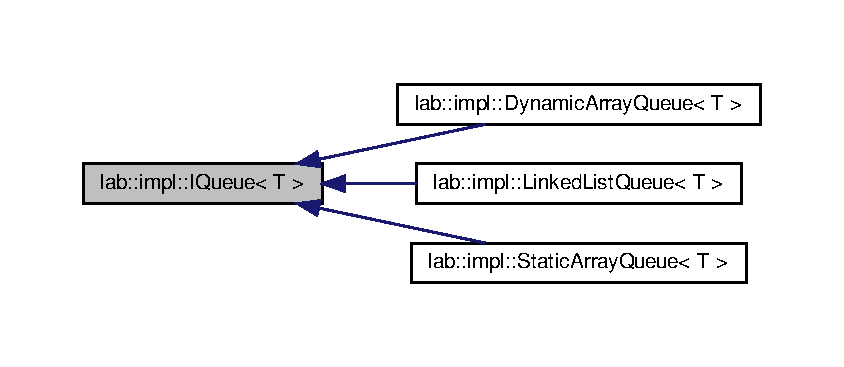
\includegraphics[width=350pt]{classlab_1_1impl_1_1IQueue__inherit__graph}
\end{center}
\end{figure}
\subsection*{Public Types}
\begin{DoxyCompactItemize}
\item 
\mbox{\Hypertarget{classlab_1_1impl_1_1IQueue_ada5c0aea26506e96fca44bf54d7ee7c1}\label{classlab_1_1impl_1_1IQueue_ada5c0aea26506e96fca44bf54d7ee7c1}} 
using {\bfseries value\+\_\+type} = T
\end{DoxyCompactItemize}
\subsection*{Public Member Functions}
\begin{DoxyCompactItemize}
\item 
\mbox{\Hypertarget{classlab_1_1impl_1_1IQueue_a9556cf62ce5ef96627fa2c2781615aab}\label{classlab_1_1impl_1_1IQueue_a9556cf62ce5ef96627fa2c2781615aab}} 
virtual void \hyperlink{classlab_1_1impl_1_1IQueue_a9556cf62ce5ef96627fa2c2781615aab}{push} (const T \&value)=0
\begin{DoxyCompactList}\small\item\em Inserts value to end of the queue. \end{DoxyCompactList}\item 
\mbox{\Hypertarget{classlab_1_1impl_1_1IQueue_a27c506405003a4b28bbd2c1a57589dad}\label{classlab_1_1impl_1_1IQueue_a27c506405003a4b28bbd2c1a57589dad}} 
virtual void \hyperlink{classlab_1_1impl_1_1IQueue_a27c506405003a4b28bbd2c1a57589dad}{push} (T \&\&value)=0
\begin{DoxyCompactList}\small\item\em Inserts value to end of the queue. \end{DoxyCompactList}\item 
\mbox{\Hypertarget{classlab_1_1impl_1_1IQueue_abdb1a94620a77e5a193b0c7ed742232f}\label{classlab_1_1impl_1_1IQueue_abdb1a94620a77e5a193b0c7ed742232f}} 
virtual T \hyperlink{classlab_1_1impl_1_1IQueue_abdb1a94620a77e5a193b0c7ed742232f}{pop} ()=0
\begin{DoxyCompactList}\small\item\em Removes first element in queue. \end{DoxyCompactList}\item 
\mbox{\Hypertarget{classlab_1_1impl_1_1IQueue_a4b0c950ff62dba782584a969e788f5a5}\label{classlab_1_1impl_1_1IQueue_a4b0c950ff62dba782584a969e788f5a5}} 
virtual const T \& \hyperlink{classlab_1_1impl_1_1IQueue_a4b0c950ff62dba782584a969e788f5a5}{front} () const =0
\begin{DoxyCompactList}\small\item\em Returns first element in queue. \end{DoxyCompactList}\item 
\mbox{\Hypertarget{classlab_1_1impl_1_1IQueue_a593e9263fbdcf840a05a21c6d8126213}\label{classlab_1_1impl_1_1IQueue_a593e9263fbdcf840a05a21c6d8126213}} 
virtual bool \hyperlink{classlab_1_1impl_1_1IQueue_a593e9263fbdcf840a05a21c6d8126213}{empty} () const noexcept=0
\begin{DoxyCompactList}\small\item\em Returns true if queue is empty. \end{DoxyCompactList}\end{DoxyCompactItemize}


\subsection{Detailed Description}
\subsubsection*{template$<$typename T$>$\newline
class lab\+::impl\+::\+I\+Queue$<$ T $>$}

Interface for queue implementations. 

The documentation for this class was generated from the following file\+:\begin{DoxyCompactItemize}
\item 
/home/starquell/\+C++/labs/4th\+Sem/lab1/src/Queue\+Interface.\+hpp\end{DoxyCompactItemize}

\hypertarget{classlab_1_1impl_1_1LinkedListQueue}{}\section{lab\+:\+:impl\+:\+:Linked\+List\+Queue$<$ T $>$ Class Template Reference}
\label{classlab_1_1impl_1_1LinkedListQueue}\index{lab\+::impl\+::\+Linked\+List\+Queue$<$ T $>$@{lab\+::impl\+::\+Linked\+List\+Queue$<$ T $>$}}


Class that holds queue implementation based on std\+::list {\bfseries Operations} complexity\+:  




{\ttfamily \#include $<$Linked\+List.\+hpp$>$}



Inheritance diagram for lab\+:\+:impl\+:\+:Linked\+List\+Queue$<$ T $>$\+:
\nopagebreak
\begin{figure}[H]
\begin{center}
\leavevmode
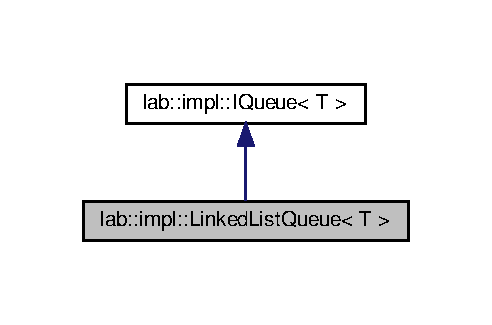
\includegraphics[width=236pt]{classlab_1_1impl_1_1LinkedListQueue__inherit__graph}
\end{center}
\end{figure}


Collaboration diagram for lab\+:\+:impl\+:\+:Linked\+List\+Queue$<$ T $>$\+:
\nopagebreak
\begin{figure}[H]
\begin{center}
\leavevmode
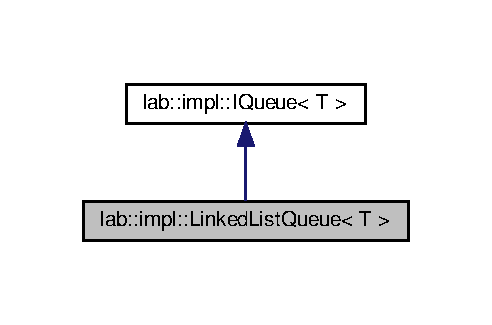
\includegraphics[width=236pt]{classlab_1_1impl_1_1LinkedListQueue__coll__graph}
\end{center}
\end{figure}
\subsection*{Public Member Functions}
\begin{DoxyCompactItemize}
\item 
{\footnotesize template$<$typename... Ts$>$ }\\\hyperlink{classlab_1_1impl_1_1LinkedListQueue_a6fbacc0f7c5c741b048326c73b761b36}{Linked\+List\+Queue} (Ts \&\&... args)
\begin{DoxyCompactList}\small\item\em Constructs queue from arbitary number of args. \end{DoxyCompactList}\item 
\mbox{\Hypertarget{classlab_1_1impl_1_1LinkedListQueue_a634f14f772cb0d9ce0a9a60a5cd81405}\label{classlab_1_1impl_1_1LinkedListQueue_a634f14f772cb0d9ce0a9a60a5cd81405}} 
void \hyperlink{classlab_1_1impl_1_1LinkedListQueue_a634f14f772cb0d9ce0a9a60a5cd81405}{push} (const T \&value) override
\begin{DoxyCompactList}\small\item\em Inserts value to end of the queue. \end{DoxyCompactList}\item 
\mbox{\Hypertarget{classlab_1_1impl_1_1LinkedListQueue_a0d57b7b5ab370206ac3e0da143c70d50}\label{classlab_1_1impl_1_1LinkedListQueue_a0d57b7b5ab370206ac3e0da143c70d50}} 
void \hyperlink{classlab_1_1impl_1_1LinkedListQueue_a0d57b7b5ab370206ac3e0da143c70d50}{push} (T \&\&value) override
\begin{DoxyCompactList}\small\item\em Inserts value to end of the queue. \end{DoxyCompactList}\item 
\mbox{\Hypertarget{classlab_1_1impl_1_1LinkedListQueue_a79a798c1277bb38a085f5f5f00f22cc3}\label{classlab_1_1impl_1_1LinkedListQueue_a79a798c1277bb38a085f5f5f00f22cc3}} 
T \hyperlink{classlab_1_1impl_1_1LinkedListQueue_a79a798c1277bb38a085f5f5f00f22cc3}{pop} () override
\begin{DoxyCompactList}\small\item\em Removes first element in queue. \end{DoxyCompactList}\item 
\mbox{\Hypertarget{classlab_1_1impl_1_1LinkedListQueue_ae2e4c57fbf4668aa7a2a9360d7dad1fc}\label{classlab_1_1impl_1_1LinkedListQueue_ae2e4c57fbf4668aa7a2a9360d7dad1fc}} 
const T \& \hyperlink{classlab_1_1impl_1_1LinkedListQueue_ae2e4c57fbf4668aa7a2a9360d7dad1fc}{front} () const override
\begin{DoxyCompactList}\small\item\em Returns first element in queue. \end{DoxyCompactList}\item 
\mbox{\Hypertarget{classlab_1_1impl_1_1LinkedListQueue_a5fa5d5a7aa41d1bcb1e034fd149c1d5b}\label{classlab_1_1impl_1_1LinkedListQueue_a5fa5d5a7aa41d1bcb1e034fd149c1d5b}} 
bool \hyperlink{classlab_1_1impl_1_1LinkedListQueue_a5fa5d5a7aa41d1bcb1e034fd149c1d5b}{empty} () const noexcept override
\begin{DoxyCompactList}\small\item\em Returns true if queue is empty. \end{DoxyCompactList}\end{DoxyCompactItemize}
\subsection*{Additional Inherited Members}


\subsection{Detailed Description}
\subsubsection*{template$<$typename T$>$\newline
class lab\+::impl\+::\+Linked\+List\+Queue$<$ T $>$}

Class that holds queue implementation based on std\+::list {\bfseries Operations} complexity\+: 

\begin{DoxyItemize}
\item Push -\/ O(1) \item Pop -\/ O(1) \end{DoxyItemize}


\subsection{Constructor \& Destructor Documentation}
\mbox{\Hypertarget{classlab_1_1impl_1_1LinkedListQueue_a6fbacc0f7c5c741b048326c73b761b36}\label{classlab_1_1impl_1_1LinkedListQueue_a6fbacc0f7c5c741b048326c73b761b36}} 
\index{lab\+::impl\+::\+Linked\+List\+Queue@{lab\+::impl\+::\+Linked\+List\+Queue}!Linked\+List\+Queue@{Linked\+List\+Queue}}
\index{Linked\+List\+Queue@{Linked\+List\+Queue}!lab\+::impl\+::\+Linked\+List\+Queue@{lab\+::impl\+::\+Linked\+List\+Queue}}
\subsubsection{\texorpdfstring{Linked\+List\+Queue()}{LinkedListQueue()}}
{\footnotesize\ttfamily template$<$typename T $>$ \\
template$<$typename... Ts$>$ \\
\hyperlink{classlab_1_1impl_1_1LinkedListQueue}{lab\+::impl\+::\+Linked\+List\+Queue}$<$ T $>$\+::\hyperlink{classlab_1_1impl_1_1LinkedListQueue}{Linked\+List\+Queue} (\begin{DoxyParamCaption}\item[{Ts \&\&...}]{args }\end{DoxyParamCaption})}



Constructs queue from arbitary number of args. 


\begin{DoxyParams}{Parameters}
{\em Args} & must be same type \\
\hline
\end{DoxyParams}


The documentation for this class was generated from the following file\+:\begin{DoxyCompactItemize}
\item 
/home/starquell/\+C++/labs/4th\+Sem/lab1/src/Linked\+List.\+hpp\end{DoxyCompactItemize}

\hypertarget{classlab_1_1Queue}{}\section{lab\+:\+:Queue$<$ T, Storage\+Type, Size\+For\+Static\+Storage $>$ Class Template Reference}
\label{classlab_1_1Queue}\index{lab\+::\+Queue$<$ T, Storage\+Type, Size\+For\+Static\+Storage $>$@{lab\+::\+Queue$<$ T, Storage\+Type, Size\+For\+Static\+Storage $>$}}


Class with queue implementation based on {\ttfamily Storage\+Type}.  




{\ttfamily \#include $<$Queue.\+hpp$>$}



Inheritance diagram for lab\+:\+:Queue$<$ T, Storage\+Type, Size\+For\+Static\+Storage $>$\+:
\nopagebreak
\begin{figure}[H]
\begin{center}
\leavevmode
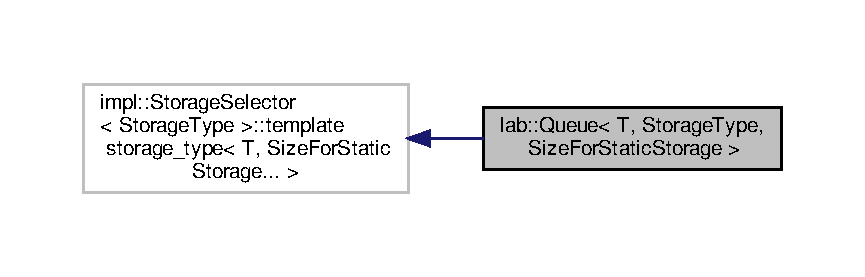
\includegraphics[width=350pt]{classlab_1_1Queue__inherit__graph}
\end{center}
\end{figure}


Collaboration diagram for lab\+:\+:Queue$<$ T, Storage\+Type, Size\+For\+Static\+Storage $>$\+:
\nopagebreak
\begin{figure}[H]
\begin{center}
\leavevmode
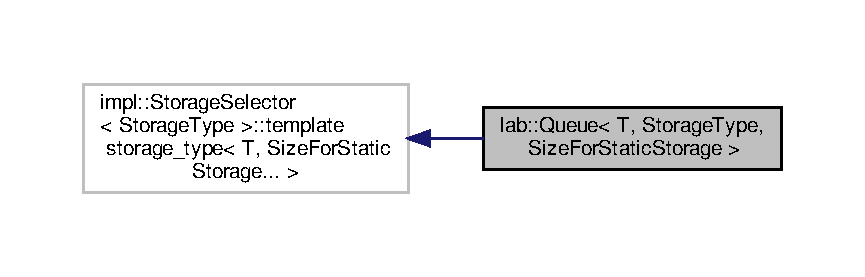
\includegraphics[width=350pt]{classlab_1_1Queue__coll__graph}
\end{center}
\end{figure}
\subsection*{Public Member Functions}
\begin{DoxyCompactItemize}
\item 
{\footnotesize template$<$typename... Ts$>$ }\\\hyperlink{classlab_1_1Queue_ae4b1fd4f3c92ac1ea001777879e87c58}{Queue} (Ts \&\&... args)
\begin{DoxyCompactList}\small\item\em Constructs queue from arbitary number of args. \end{DoxyCompactList}\end{DoxyCompactItemize}


\subsection{Detailed Description}
\subsubsection*{template$<$typename T, Storage Storage\+Type = Storage\+::\+Linked\+List, std\+::size\+\_\+t... Size\+For\+Static\+Storage$>$\newline
class lab\+::\+Queue$<$ T, Storage\+Type, Size\+For\+Static\+Storage $>$}

Class with queue implementation based on {\ttfamily Storage\+Type}. 

\begin{DoxyAttention}{Attention}
Use 
\end{DoxyAttention}

\begin{DoxyParams}{Parameters}
{\em Size\+For\+Static\+Storage} & to set max queue size if Storage\+Type == Static \\
\hline
\end{DoxyParams}


\subsection{Constructor \& Destructor Documentation}
\mbox{\Hypertarget{classlab_1_1Queue_ae4b1fd4f3c92ac1ea001777879e87c58}\label{classlab_1_1Queue_ae4b1fd4f3c92ac1ea001777879e87c58}} 
\index{lab\+::\+Queue@{lab\+::\+Queue}!Queue@{Queue}}
\index{Queue@{Queue}!lab\+::\+Queue@{lab\+::\+Queue}}
\subsubsection{\texorpdfstring{Queue()}{Queue()}}
{\footnotesize\ttfamily template$<$typename T , Storage Storage\+Type = Storage\+::\+Linked\+List, std\+::size\+\_\+t... Size\+For\+Static\+Storage$>$ \\
template$<$typename... Ts$>$ \\
\hyperlink{classlab_1_1Queue}{lab\+::\+Queue}$<$ T, Storage\+Type, Size\+For\+Static\+Storage $>$\+::\hyperlink{classlab_1_1Queue}{Queue} (\begin{DoxyParamCaption}\item[{Ts \&\&...}]{args }\end{DoxyParamCaption})\hspace{0.3cm}{\ttfamily [inline]}}



Constructs queue from arbitary number of args. 


\begin{DoxyParams}{Parameters}
{\em Args} & must be same type \\
\hline
\end{DoxyParams}


The documentation for this class was generated from the following file\+:\begin{DoxyCompactItemize}
\item 
/home/starquell/\+C++/labs/4th\+Sem/lab1/src/Queue.\+hpp\end{DoxyCompactItemize}

\hypertarget{classlab_1_1impl_1_1StaticArrayQueue}{}\section{lab\+:\+:impl\+:\+:Static\+Array\+Queue$<$ T, Size $>$ Class Template Reference}
\label{classlab_1_1impl_1_1StaticArrayQueue}\index{lab\+::impl\+::\+Static\+Array\+Queue$<$ T, Size $>$@{lab\+::impl\+::\+Static\+Array\+Queue$<$ T, Size $>$}}


Class that holds queue implementation based on std\+::array {\bfseries Operations} complexity\+:  




{\ttfamily \#include $<$Static\+Array.\+hpp$>$}



Inheritance diagram for lab\+:\+:impl\+:\+:Static\+Array\+Queue$<$ T, Size $>$\+:
\nopagebreak
\begin{figure}[H]
\begin{center}
\leavevmode
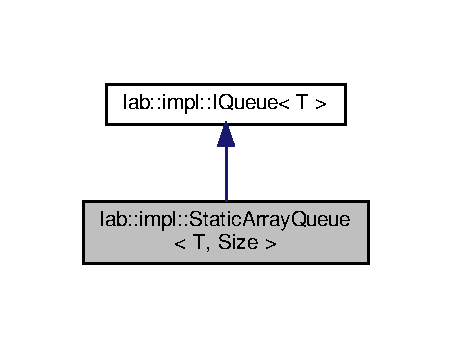
\includegraphics[width=217pt]{classlab_1_1impl_1_1StaticArrayQueue__inherit__graph}
\end{center}
\end{figure}


Collaboration diagram for lab\+:\+:impl\+:\+:Static\+Array\+Queue$<$ T, Size $>$\+:
\nopagebreak
\begin{figure}[H]
\begin{center}
\leavevmode
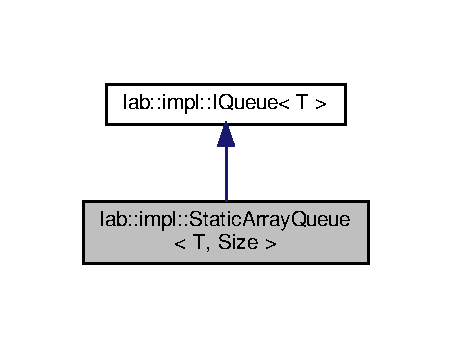
\includegraphics[width=217pt]{classlab_1_1impl_1_1StaticArrayQueue__coll__graph}
\end{center}
\end{figure}
\subsection*{Public Member Functions}
\begin{DoxyCompactItemize}
\item 
{\footnotesize template$<$typename... Args$>$ }\\\hyperlink{classlab_1_1impl_1_1StaticArrayQueue_a8c77c1506a3fdc3c4b0ccd41aa7352ff}{Static\+Array\+Queue} (Args \&\&... args)
\begin{DoxyCompactList}\small\item\em Constructs queue from arbitary number of args. \end{DoxyCompactList}\item 
\mbox{\Hypertarget{classlab_1_1impl_1_1StaticArrayQueue_a73094b978df25af0453d5e9787d81957}\label{classlab_1_1impl_1_1StaticArrayQueue_a73094b978df25af0453d5e9787d81957}} 
void \hyperlink{classlab_1_1impl_1_1StaticArrayQueue_a73094b978df25af0453d5e9787d81957}{push} (const T \&value) override
\begin{DoxyCompactList}\small\item\em Inserts value to end of the queue. \end{DoxyCompactList}\item 
\mbox{\Hypertarget{classlab_1_1impl_1_1StaticArrayQueue_a55460501294a71b11e94c44bfcdb18d3}\label{classlab_1_1impl_1_1StaticArrayQueue_a55460501294a71b11e94c44bfcdb18d3}} 
void \hyperlink{classlab_1_1impl_1_1StaticArrayQueue_a55460501294a71b11e94c44bfcdb18d3}{push} (T \&\&value) override
\begin{DoxyCompactList}\small\item\em Inserts value to end of the queue. \end{DoxyCompactList}\item 
\mbox{\Hypertarget{classlab_1_1impl_1_1StaticArrayQueue_ad246e9b69d05aa6705b796a27082a1a4}\label{classlab_1_1impl_1_1StaticArrayQueue_ad246e9b69d05aa6705b796a27082a1a4}} 
T \hyperlink{classlab_1_1impl_1_1StaticArrayQueue_ad246e9b69d05aa6705b796a27082a1a4}{pop} () override
\begin{DoxyCompactList}\small\item\em Removes first element in queue. \end{DoxyCompactList}\item 
\mbox{\Hypertarget{classlab_1_1impl_1_1StaticArrayQueue_adbf6d2a433d6dcf637fadfd555df4dbd}\label{classlab_1_1impl_1_1StaticArrayQueue_adbf6d2a433d6dcf637fadfd555df4dbd}} 
const T \& \hyperlink{classlab_1_1impl_1_1StaticArrayQueue_adbf6d2a433d6dcf637fadfd555df4dbd}{front} () const override
\begin{DoxyCompactList}\small\item\em Returns first element in queue. \end{DoxyCompactList}\item 
\mbox{\Hypertarget{classlab_1_1impl_1_1StaticArrayQueue_ad4488385381fe0920676ce45e221e4b5}\label{classlab_1_1impl_1_1StaticArrayQueue_ad4488385381fe0920676ce45e221e4b5}} 
bool \hyperlink{classlab_1_1impl_1_1StaticArrayQueue_ad4488385381fe0920676ce45e221e4b5}{empty} () const noexcept override
\begin{DoxyCompactList}\small\item\em Returns true if queue is empty. \end{DoxyCompactList}\end{DoxyCompactItemize}
\subsection*{Additional Inherited Members}


\subsection{Detailed Description}
\subsubsection*{template$<$typename T, std\+::size\+\_\+t Size$>$\newline
class lab\+::impl\+::\+Static\+Array\+Queue$<$ T, Size $>$}

Class that holds queue implementation based on std\+::array {\bfseries Operations} complexity\+: 

\begin{DoxyItemize}
\item Push -\/ O(1) \item Pop -\/ O(1) \end{DoxyItemize}


\subsection{Constructor \& Destructor Documentation}
\mbox{\Hypertarget{classlab_1_1impl_1_1StaticArrayQueue_a8c77c1506a3fdc3c4b0ccd41aa7352ff}\label{classlab_1_1impl_1_1StaticArrayQueue_a8c77c1506a3fdc3c4b0ccd41aa7352ff}} 
\index{lab\+::impl\+::\+Static\+Array\+Queue@{lab\+::impl\+::\+Static\+Array\+Queue}!Static\+Array\+Queue@{Static\+Array\+Queue}}
\index{Static\+Array\+Queue@{Static\+Array\+Queue}!lab\+::impl\+::\+Static\+Array\+Queue@{lab\+::impl\+::\+Static\+Array\+Queue}}
\subsubsection{\texorpdfstring{Static\+Array\+Queue()}{StaticArrayQueue()}}
{\footnotesize\ttfamily template$<$typename T , std\+::size\+\_\+t Size$>$ \\
template$<$typename... Args$>$ \\
\hyperlink{classlab_1_1impl_1_1StaticArrayQueue}{lab\+::impl\+::\+Static\+Array\+Queue}$<$ T, Size $>$\+::\hyperlink{classlab_1_1impl_1_1StaticArrayQueue}{Static\+Array\+Queue} (\begin{DoxyParamCaption}\item[{Args \&\&...}]{args }\end{DoxyParamCaption})}



Constructs queue from arbitary number of args. 


\begin{DoxyParams}{Parameters}
{\em Args} & must be same type \\
\hline
\end{DoxyParams}


The documentation for this class was generated from the following file\+:\begin{DoxyCompactItemize}
\item 
/home/starquell/\+C++/labs/4th\+Sem/lab1/src/Static\+Array.\+hpp\end{DoxyCompactItemize}

\hypertarget{structlab_1_1impl_1_1StorageSelector}{}\section{lab\+:\+:impl\+:\+:Storage\+Selector$<$ storage $>$ Struct Template Reference}
\label{structlab_1_1impl_1_1StorageSelector}\index{lab\+::impl\+::\+Storage\+Selector$<$ storage $>$@{lab\+::impl\+::\+Storage\+Selector$<$ storage $>$}}
\subsection*{Public Types}
\begin{DoxyCompactItemize}
\item 
\mbox{\Hypertarget{structlab_1_1impl_1_1StorageSelector_ad8ace3a7105ad30f2ea40798b2d56934}\label{structlab_1_1impl_1_1StorageSelector_ad8ace3a7105ad30f2ea40798b2d56934}} 
using {\bfseries storage\+\_\+type} = \hyperlink{classlab_1_1impl_1_1UndefinedStorage}{Undefined\+Storage}
\end{DoxyCompactItemize}


The documentation for this struct was generated from the following file\+:\begin{DoxyCompactItemize}
\item 
/home/starquell/\+C++/labs/4th\+Sem/lab1/src/Queue.\+hpp\end{DoxyCompactItemize}

\hypertarget{structlab_1_1impl_1_1StorageSelector_3_01Storage_1_1Dynamic_01_4}{}\section{lab\+:\+:impl\+:\+:Storage\+Selector$<$ Storage\+:\+:Dynamic $>$ Struct Template Reference}
\label{structlab_1_1impl_1_1StorageSelector_3_01Storage_1_1Dynamic_01_4}\index{lab\+::impl\+::\+Storage\+Selector$<$ Storage\+::\+Dynamic $>$@{lab\+::impl\+::\+Storage\+Selector$<$ Storage\+::\+Dynamic $>$}}
\subsection*{Public Types}
\begin{DoxyCompactItemize}
\item 
\mbox{\Hypertarget{structlab_1_1impl_1_1StorageSelector_3_01Storage_1_1Dynamic_01_4_ace5d3014667be4ed39cfafcaf4882a5d}\label{structlab_1_1impl_1_1StorageSelector_3_01Storage_1_1Dynamic_01_4_ace5d3014667be4ed39cfafcaf4882a5d}} 
{\footnotesize template$<$typename T $>$ }\\using {\bfseries storage\+\_\+type} = \hyperlink{classlab_1_1impl_1_1DynamicArrayQueue}{impl\+::\+Dynamic\+Array\+Queue}$<$ T $>$
\end{DoxyCompactItemize}


The documentation for this struct was generated from the following file\+:\begin{DoxyCompactItemize}
\item 
/home/starquell/\+C++/labs/4th\+Sem/lab1/src/Queue.\+hpp\end{DoxyCompactItemize}

\hypertarget{structlab_1_1impl_1_1StorageSelector_3_01Storage_1_1LinkedList_01_4}{}\section{lab\+:\+:impl\+:\+:Storage\+Selector$<$ Storage\+:\+:Linked\+List $>$ Struct Template Reference}
\label{structlab_1_1impl_1_1StorageSelector_3_01Storage_1_1LinkedList_01_4}\index{lab\+::impl\+::\+Storage\+Selector$<$ Storage\+::\+Linked\+List $>$@{lab\+::impl\+::\+Storage\+Selector$<$ Storage\+::\+Linked\+List $>$}}
\subsection*{Public Types}
\begin{DoxyCompactItemize}
\item 
\mbox{\Hypertarget{structlab_1_1impl_1_1StorageSelector_3_01Storage_1_1LinkedList_01_4_ad2ccdeed322a59cd3bbcba25444972ec}\label{structlab_1_1impl_1_1StorageSelector_3_01Storage_1_1LinkedList_01_4_ad2ccdeed322a59cd3bbcba25444972ec}} 
{\footnotesize template$<$typename T $>$ }\\using {\bfseries storage\+\_\+type} = \hyperlink{classlab_1_1impl_1_1LinkedListQueue}{impl\+::\+Linked\+List\+Queue}$<$ T $>$
\end{DoxyCompactItemize}


The documentation for this struct was generated from the following file\+:\begin{DoxyCompactItemize}
\item 
/home/starquell/\+C++/labs/4th\+Sem/lab1/src/Queue.\+hpp\end{DoxyCompactItemize}

\hypertarget{structlab_1_1impl_1_1StorageSelector_3_01Storage_1_1Static_01_4}{}\section{lab\+:\+:impl\+:\+:Storage\+Selector$<$ Storage\+:\+:Static $>$ Struct Template Reference}
\label{structlab_1_1impl_1_1StorageSelector_3_01Storage_1_1Static_01_4}\index{lab\+::impl\+::\+Storage\+Selector$<$ Storage\+::\+Static $>$@{lab\+::impl\+::\+Storage\+Selector$<$ Storage\+::\+Static $>$}}
\subsection*{Public Types}
\begin{DoxyCompactItemize}
\item 
\mbox{\Hypertarget{structlab_1_1impl_1_1StorageSelector_3_01Storage_1_1Static_01_4_a16cc53047e6db12365451ff2de980037}\label{structlab_1_1impl_1_1StorageSelector_3_01Storage_1_1Static_01_4_a16cc53047e6db12365451ff2de980037}} 
{\footnotesize template$<$typename T , std\+::size\+\_\+t Size\+For\+Static$>$ }\\using {\bfseries storage\+\_\+type} = \hyperlink{classlab_1_1impl_1_1StaticArrayQueue}{impl\+::\+Static\+Array\+Queue}$<$ T, Size\+For\+Static $>$
\end{DoxyCompactItemize}


The documentation for this struct was generated from the following file\+:\begin{DoxyCompactItemize}
\item 
/home/starquell/\+C++/labs/4th\+Sem/lab1/src/Queue.\+hpp\end{DoxyCompactItemize}

\hypertarget{classlab_1_1impl_1_1UndefinedStorage}{}\section{lab\+:\+:impl\+:\+:Undefined\+Storage Class Reference}
\label{classlab_1_1impl_1_1UndefinedStorage}\index{lab\+::impl\+::\+Undefined\+Storage@{lab\+::impl\+::\+Undefined\+Storage}}


The documentation for this class was generated from the following file\+:\begin{DoxyCompactItemize}
\item 
/home/starquell/\+C++/labs/4th\+Sem/lab1/src/Queue.\+hpp\end{DoxyCompactItemize}

%--- End generated contents ---

% Index
\backmatter
\newpage
\phantomsection
\clearemptydoublepage
\addcontentsline{toc}{chapter}{Index}
\printindex

\end{document}
